\documentclass[a4paper]{article} % A4 paper and 11pt font size

\usepackage{braket}
\usepackage{amsmath}
\usepackage{amssymb}
\usepackage{bm}
\usepackage[utf8]{inputenc}
\usepackage{verbatim}
\usepackage{tikz}
%\usepackage{tikz-feynman}
\usepackage{pgfplots}
\usepackage{pgffor}
\usepackage[version-1-compatibility]{siunitx}
\usepackage{fancyhdr}

\newcommand{\sech}{\text{sech}}
\newcommand{\vect}[1]{\mathbf{#1}}


\usepackage{hyperref}

\usepackage{geometry}

 \geometry{
 a4paper,
 total={210mm,297mm},
 left=28mm,
 right=28mm,
 top=30mm,
 bottom=40mm,
 }


\usepackage{framed}

\usepackage{amssymb} %for Lagrangian L, order O
\usepackage{cancel} %for strikethroughs
\usepackage{slashed} %for Feynman slashes

\newcommand{\me}{\mathrm{e}}
\newcommand{\D}{\mathcal{D}}
\newcommand{\pmx}[1]{\begin{pmatrix}#1\end{pmatrix}}
\newcommand{\m}{\mathcal{M}}
\newcommand{\br}{\mathcal{B}}
\DeclareMathOperator{\im}{Im}
\DeclareMathOperator{\re}{Re}

\newcommand{\bpp}{\(B^0 \to \pi^+\pi^-\)}
\newcommand{\bpk}{\(B^0 \to \phi K_S\)}
\newcommand{\tr}[1]{\text{Tr}\left[#1\right]}
\newcommand{\mev}{\text{ MeV}}
\newcommand{\gev}{\text{ GeV}}

\renewcommand{\c}{\mathcal{C}}
\newcommand{\p}{\mathcal{P}}

\usepackage{gensymb}

\usepackage{fancyhdr}
\usepackage{pdflscape}
\usepackage{bm}

%for side-by-side figures
\usepackage{graphicx}
\usepackage{caption}
\usepackage{subcaption}


%Curly epsilons
\let\oldepsilon\epsilon
\let\epsilon\varepsilon


\setlength{\parindent}{2em}
\setlength{\parskip}{1em}
\renewcommand{\baselinestretch}{1.1}

%----------------------------------------------------------------------------------------
%	TITLE SECTION
%----------------------------------------------------------------------------------------
\setlength\parindent{0pt} % Removes all indentation from paragraphs - comment this line for an assignment with lots of text


\pagenumbering{arabic}
\begin{document}
\pagestyle{empty}

\newcommand{\HRule}{\rule{\linewidth}{0.5mm}}

\begin{titlepage}

    \begin{center}
        \textsc{\large SN: 587623}\\[6cm]

        \HRule \\[0.5cm]
		\Huge \textbf{PHYC90012 General Relativity}\\[0.5cm]
        \huge \textbf{Assignment 1}\\[0.5cm] 
        \HRule \\[1.5cm]
        \begin{minipage}{0.4\textwidth}
        \begin{center}

        \large By \\[0.75cm]
        \huge Braden \scshape Moore \\[0.5cm]
        \normalsize \normalfont Master of Science \\
        The University of Melbourne \\

        \end{center}
        \end{minipage}

        \vfill

        \large \today
    \end{center}

\newpage
\end{titlepage}
%----------------------------------------------------------------------------------------
\pagestyle{fancy}
\pagenumbering{arabic}
\rfoot{\textsc{Braden Moore, 587623}}
\lfoot{\textsc{\today}}
\rhead{\textsc{General Relativity: Assignment 1}}
\setcounter{page}{1}
\section{Drag racing in space in the Greco-Roman era}
%%%%%%%%%%%%%%%%%%%%QUESTION 1%%%%%%%%%%%%%%%%%%%%%
\begin{framed}
Buoyed by the success of their intrepid interstellar experiment on the twin paradox (the legend is recounted in Section 1.13 of the 1st edition of A First Course in General Relativity, by B. F. Schutz), twin sisters Artemis and Diana decide to conduct a follow-up investigation into the physics of accelerated reference frames in flat space as follows. At the same instant, 1 the sisters jump into two rocket ships, which are initially at rest in a global inertial frame, 2 and race off in the x-direction with constant but unequal proper accelerations. In their space packs they carry a laser pointer (Artemis), a mirror (Diana), and identically manufactured clocks and rulers (Artemis and Diana). 3 Their departure points and trajectories are not the same. In the global inertial frame in which the rocket ships are initially at rest, Artemis starts out from the event $(t, x, y, z) = (0, g^{-1}, 0, 0)$, where $(t, x, y, z)$ are standard Minkowski coordinates, and g denotes her proper acceleration. As derived in lectures, her trajectory on a spacetime diagram is a hyperbola in the x-t plane defined parametrically by
\begin{align}
t_A(\tau A) &= g^{-1} \sinh g\tau_A,\label{eq1}\\
x_A(\tau A) &= g^{-1} \cosh g\tau_A,\label{eq2}\\
y_A(\tau A) &= 0,\\
z_A(\tau A) &= 0
\end{align}

where $\tau_A$ is her proper time. Diana’s departure point, trajectory, and proper acceleration remain unspecified for now.
\end{framed}

\begin{framed}
\textbf{(a)}
Before attempting any experiments, Artemis constructs a new coordinate system $(t, x, y, z)$ for making measurements in the neighbourhood of her rocket ship. The construction proceeds in three steps, which we copy here. 
\end{framed}

\begin{framed}
\textbf{i.} 
Fermi-Walker transport the Minkowski basis vectors $\vec{e}_0$, $\vec{e}_1$, $\vec{e}_2$, and $\vec{e}_3$ along Artemis’s world line. Show that this procedure yields a new basis
\begin{align}
\vec{e}_0(\tau_A) &= \vec{e}_0 \cosh g\tau_A +\vec{e}_1 \sinh g\tau_A,\label{ai. eq1}\\
\vec{e}_1(\tau_A) &= \vec{e}_0 \sinh g\tau_A +\vec{e}_1 \cosh g\tau_A,\\
\vec{e}_2(\tau_A) &= \vec{e}_2,\\
\vec{e}_3(\tau_A) &= \vec{e}_3\label{ai. eq4}
\end{align}

at the point along the world line labelled by $\tau_A$.
\end{framed}

A Fermi-Walker transported basis in unprimed coordinates (i.e. the global inertial reference frame; Minkowski coordinates) $\vec{e}$ satisfies the equation
\begin{equation}
\frac{d\vec{e}_{\alpha}}{d\tau_A}=\vec{u}(\vec{a}\cdot\vec{e}_{\alpha})-\vec{a}(\vec{u}\cdot\vec{e}_{\alpha})
\end{equation}
with Christoffel symbols all equivalently zero. Starting from Artemis' position vector $\vec{x}$,

\begin{align}
\vec{x}(\tau_A)&=(g^{-1}\sinh g\tau_A,g^{-1}\cosh g\tau_A,0,0)\\
\Rightarrow \vec{u}=\frac{d\vec{x}}{d\tau_A}&=(\cosh g\tau_A,\sinh g\tau_A,0,0)\\
\vec{a}&=\frac{d\vec{u}}{d\tau}\quad\text{in flat space}\\
&=(g\sinh g\tau_A,g\cosh g\tau_A,0,0)\\
\Rightarrow \frac{d\vec{e}_0}{d\tau_A}&=(\cosh g\tau_A,\sinh g\tau_A,0,0)\cdot(-g\sinh g\tau_A)
-(g\sinh g\tau_A, g\cosh g\tau_A,0,0)\cdot(-\cosh g\tau_A)\\
&=g\left[(\sinh g\tau_A \cdot \cosh g\tau_A,\cosh^2 g\tau_A,0,0)-(\sinh g\tau_A \cdot \cosh g\tau_A,\sinh^2 g\tau_A,0,0)\right]\\
&=g(0,\underbrace{\cosh^2 g\tau_A-\sinh^2 g\tau_A}_{=1},0,0)\\
&=g(0,1,0,0)\\
&=g\vec{e}_1 \label{de0dtau}
\intertext{Similarly,}
\frac{d\vec{e}_1}{d\tau_A}&=(\cosh g\tau_A,\sinh g\tau_A,0,0)\cdot(g \cosh g\tau_A)
-(g\sinh g\tau_A, g\cosh g\tau_A,0,0)\cdot(\sinh g\tau_A)\\
&=g\left[(\cosh^2 g\tau_A,\sinh g\tau_A \cdot \cosh g\tau_A,0,0)
-(\sinh^2 g\tau_A,\sinh g\tau_A \cdot \cosh g\tau_A,0,0)\right]\\
&=g(\underbrace{\cosh^2 g\tau_A-\sinh^2 g\tau_A}_{=1},0,0,0)\\
&=g(1,0,0,0)\\
&=g\vec{e}_0 \label{de1dtau}
\end{align}

Previously we have considered the basis vectors in Minkowski coordinates $\vec{e}_{\alpha}$. However, our primed basis must also satisfy (\ref{de0dtau}) and (\ref{de1dtau}) under Fermi-Walker transport, i.e.

\begin{align}
\frac{d\vec{e}_{0'}}{d\tau_A}&=g\vec{e}_{1'}\label{de0' dtau} \\
\frac{d\vec{e}_{1'}}{d\tau_A}&=g\vec{e}_{0'} \label{de1' dtau}
\end{align}

From (\ref{de0' dtau}) and (\ref{de1' dtau}) we have
\begin{align}
\frac{d^2\vec{e}_{0'}}{d\tau_A}&=g^2\vec{e}_{0'}\\
\frac{d^2\vec{e}_{1'}}{d\tau_A}&=g^2\vec{e}_{1'}
\end{align}
These differential equations can be solved for $\vec{e}_{0'}$ and $\vec{e}_{1'}$ 

\begin{align}
\vec{e}_{0'}^{\alpha}&=A^{\alpha}\sinh g\tau_A+B^{\alpha}\cosh g\tau_A \label{e0' consts} \\
\vec{e}_{1'}^{\alpha}&=C^{\alpha}\sinh g\tau_A+D^{\alpha}\cosh g\tau_A \label{e1' consts}
\end{align}

Combining (\ref{de0' dtau}) with (\ref{e1' consts}) we find
\begin{equation}
A^{\alpha}\cosh g\tau_A + B^{\alpha}\sinh g\tau_A=C^{\alpha}\sinh g\tau_A+D^{\alpha}\cosh g\tau_A
\end{equation}

\begin{align}
\Rightarrow A^{\alpha}&=D^{\alpha}\\
B^{\alpha}&=C^{\alpha}
\intertext{and so we have}
\vec{e}_{0'}&=A^{\alpha}\sinh g\tau_A+B^{\alpha}\cosh g\tau_A\\
\vec{e}_{1'}&=B^{\alpha}\sinh g \tau_A+A^{\alpha}\cosh g \tau_A
\end{align}

At $t=\tau_A=0$, the basis vectors of the primed and unprimed frames are equivalent. So for $\tau_A=0 \Rightarrow \vec{e}_{0}=\vec{e}_{0'}$, with $\sinh 0 =0$ and $\cosh 0 =1$ we have
\begin{align}
\Rightarrow 1&=B^{0}\\
0&=B^{1}\\
0&=B^{2}\\
0&=B^{3}\Rightarrow B^{i}=0,\text{ where }i=1,2,3
\end{align}

Applying a similar treatment for $\vec{e}_{1}=\vec{e}_{1'}$,
\begin{align}
0&=A^{0}\\
1&=A^{1}\\
0&=A^{2}\\
0&=A^{3}
\end{align}
which gives us $A^{1}=1$ and $A^{0,2,3}=0$.

Using these results with (\ref{e0' consts}) and (\ref{e1' consts}) we conclude
\begin{align}
\vec{e}_{0'}&=(\cosh g\tau_A,\sinh g\tau_A,0,0)=\vec{e}_0 \cosh g\tau_A+\vec{e}_1 \sinh g \tau_A\\
\vec{e}_{1'}&=(\sinh g\tau_A,\cosh g\tau_A,0,0)=\vec{e}_0 \sinh g\tau_A+\vec{e}_1 \cosh g \tau_A
\end{align}
as required.


\begin{framed}
\textbf{ii.} 
Verify that one can obtain (\ref{ai. eq1})-(\ref{ai. eq4}) by Lorentz boosting the Minkowski basis vectors into the rocket ship’s momentarily comoving reference frame.
\end{framed}

Regular vectors transform like
\begin{equation}
A^{\alpha'}=\Lambda^{\alpha'}_{\beta}(v)A^{\beta}
\end{equation}

However, basis vectors transform opppositely; that is
\begin{equation}
\vec{e}_{\alpha'}=\Lambda^{\beta}_{\alpha'}\vec{e}_{\beta}
\end{equation}

Our Lorentz transform matrix $\Lambda^{\alpha'}_{\beta}$ is given by
\begin{equation}
\Lambda^{\alpha'}_{\beta}=\pmx{\lambda&-v\lambda&0&0\\
-v\lambda&\lambda&0&0\\
0&0&1&0\\
0&0&0&1}
\end{equation}
where $v$ is the velocity $\frac{dx}{dt}$ of Artemis in the unprimed frame, and $\lambda=\frac{1}{\sqrt{1-v^2}}$. However, to transform basis vectors we require the inverse matrix, which is given by
\begin{equation}
\Lambda^{\beta}_{\alpha'}=\left(\Lambda^{\alpha'}_{\beta}\right)^{-1}=\pmx{\lambda&v\lambda&0&0\\
v\lambda&\lambda&0&0\\
0&0&1&0\\
0&0&0&1}
\end{equation}

We can calculate the values of $v$ and $\lambda$ as
\begin{align}
v&=\frac{dx_A(\tau_A)}{dt_A(\tau_A)}\\
&=\frac{dx(\tau_A)}{d\tau_A}\cdot\frac{d\tau_A}{dt_A(\tau_A)}\\
&=\frac{\sinh g\tau_A}{\cosh g\tau_A}\\
&=\tanh g\tau_A\\
\lambda&=\frac{1}{\sqrt{1-v^2}}\\
&=\frac{1}{\sqrt{1-\tanh^2 g\tau_A}}\\
&=\frac{1}{\sqrt{\sech^2 g\tau}}\\
&=\frac{1}{\sech g\tau_A}\\
&=\cosh g\tau_A\\
\Rightarrow \Lambda^{\beta}_{\alpha'}&=\pmx{\cosh g\tau_A&\sinh g\tau_A&0&0\\
\sinh g\tau_A &\cosh g\tau_A&0&0\\
0&0&1&0\\
0&0&0&1}
\end{align}



Hence we Lorentz boost the basis vectors as
\begin{align}
\vec{e}_{0'}&=\Lambda^{\beta}_{0'}\vec{e}_{\beta}=\Lambda^{0}_{0'}\vec{e}_{0}+\Lambda^{1}_{0'}\vec{e}_{1}\\
&=\vec{e}_0 \cosh g\tau_A +\vec{e}_1 \sinh g\tau_A\\
\vec{e}_{1'}&=\Lambda^{\beta}_{1'}\vec{e}_{\beta}=\Lambda^{0}_{1'}\vec{e}_{0}+\Lambda^{1}_{1'}\vec{e}_{1}\\
&=\vec{e}_0 \sinh g\tau_A +\vec{e}_1 \cosh g\tau_A\\
\end{align}
as required.

\begin{framed}
\textbf{iii.} 
Let the vector $x'\vec{e}_{1'}+y'\vec{e}_{2'}+z'\vec{e}_{3'}$ be the displacement of an event $P$ from the spacetime location of the centre of mass of Artemis’s rocket ship. Let $t'$ be the proper time measured by Artemis at the space point $(x,y,z)=(0,0,0)$. Show that these definitions lead to the transformation
\begin{align}
t&=(g^{-1}+x')\sinh gt', \label{aiii eq1} \\
x&=(g^{-1}+x') \cosh gt',\\
y&=y', \\
z&=z', \label{aiii eq4}
\end{align}
if $P$ occurs at $(t,x,y,z)$ in Minkowski coordinates.
\end{framed}

\begin{figure}[h]
\centering
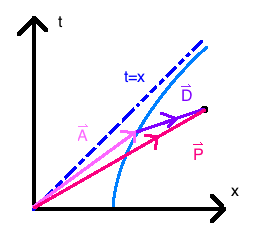
\includegraphics[width=0.5\textwidth]{images/aiii_diagram.png}
\caption{Spacetime diagram of Artemis and event P}
\label{aiii diagram}
\end{figure}

We define the vectors $\vec{A}$, $\vec{D}$ and $\vec{P}$ as
\begin{align}
\vec{A}&=\text{Artemis' position in the unprimed coordinates}\\
&=g^{-1}\sinh g\tau_A \vec{e}_0+g^{-1}\cosh g\tau_A \vec{e}_1\\
\vec{D}&=\text{displacement of an event P from Artemis' center-of-mass in the primed coordinates}\\
&=x'\sinh g\tau_A \vec{e}_0+x'\cosh g\tau_A \vec{1}+y'\vec{e}_{2}+z'\vec{e}_{3} \quad\text{from (\ref{ai. eq1})-(\ref{ai. eq4})}\\
\vec{P}&=\text{spacetime position of event P in the unprimed coordinates}\\
&=t\vec{e}_0+x\vec{e}_1+y\vec{e}_2+z\vec{e}_3
\end{align}

From Figure \ref{aiii diagram} we see that $\vec{P}=\vec{A}+\vec{D}$, hence
\begin{align}
t\vec{e}_0+x\vec{e}_1+y\vec{e}_2+z\vec{e}_3
&=\vec{e}_0(g^{-1}\sinh g\tau_A+x'\sinh g\tau_A)
+\vec{e}_1(g^{-1}\cosh g\tau_A+x'\cosh g\tau_A)+y'\vec{e}_2+z'\vec{e}_3\\
\Rightarrow t&=(g^{-1}+x')\sinh g\tau_A\\
x&=(g^{-1}+x')\cosh g\tau_A\\
y&=y'\\
z&=z'
\end{align}
as required.


\begin{framed}
\textbf{(b)} 
The primed coordinates are curvilinear, even though the spacetime is flat.
\end{framed}

\begin{framed}
\textbf{i.} Transform the Minkowski metric of the global inertial frame into the primed coordinates. You should find
\begin{equation}
g_{\alpha' \beta'}=\text{diag}[-(1+gx')^2,1,1,1].\label{primed metric}
\end{equation}
\end{framed}

The metric in primed coordinates $g_{\alpha'\beta'}$ is found from the metric in unprimed coordinates by
\begin{equation}
g_{\alpha'\beta'}=\frac{\partial x^{\alpha}}{\partial x^{\alpha'}}\frac{\partial x^{\beta}}{\partial x^{\beta'}}g_{\alpha\beta}
\end{equation}

Recall the metric $g_{\alpha\beta}$ is given by
\begin{equation}
g_{\alpha\beta}=\text{diag}(-1,1,1,1)\label{Mink metric}
\end{equation}

We can calculate $\frac{\partial x^{\alpha}}{\partial x^{\alpha'}}$ from (\ref{aiii eq1})-(\ref{aiii eq4})
\begin{equation}
\frac{\partial x^{\alpha}}{\partial x^{\alpha'}}=\pmx{(1+gx')\cosh gt'&(1+gx')\sinh gt&0&0\\
\sinh gt'& \cosh gt'&0&0\\
0&0&1&0\\
0&0&0&1} \label{bi matrix diff}
\end{equation}

Combining these equations (and omitting all zeroes for simplicity), we find
\begin{align}
g_{0'0'}&=\frac{\partial x^0}{\partial x^{0'}} \frac{\partial x^0}{\partial x^{0'}} g_{00}
+\frac{\partial x^1}{\partial x^{0'}}\frac{\partial x^1}{\partial x^{0'}}g_{11}\\
&=-(1+gx')^2\cosh^2 gt'+(1+gx')^2\sinh^2 gt'\\
&=-(1+gx')^2(\underbrace{\cosh^2 gt'-\sinh^2 gt'}_{=1})\\
&=-(1+gx')^2
\intertext{}
g_{1'1'}&=\frac{\partial x^0}{\partial x^{1'}} \frac{\partial x^0}{\partial x^{1'}} g_{00}
+\frac{\partial x^1}{\partial x^{1'}}\frac{\partial x^1}{\partial x^{1'}}g_{11}\\
&=-\sinh^2 gt'+\cosh^2 gt'\\
&=1
\intertext{}
g_{2'2'}&=\frac{\partial x^2}{\partial x^{2'}} \frac{\partial x^2}{\partial x^{2'}} g_{22}\\
&=1
\intertext{}
g_{3'3'}&=\frac{\partial x^3}{\partial x^{3'}} \frac{\partial x^3}{\partial x^{3'}} g_{33}\\
&=1
\end{align}

So we have found the diagonal terms of the primed metric. We now need to find the off-diagonal terms. We can use the symmetric property of the metric (i.e. $g_{\alpha'\beta'}=g_{\beta'\alpha'}$) to reduce the amount of effort required.

\begin{align}
g_{0'1'}&=\frac{\partial x^0}{\partial x^{0'}} \frac{\partial x^0}{\partial x^{1'}} g_{00}
+\frac{\partial x^1}{\partial x^{0'}}\frac{\partial x^1}{\partial x^{1'}}g_{11}\\
&=-(1+gx')\cosh gt' \sinh gt'+(1+gx')\sinh gt' \cosh gt'\\
&=0 \Rightarrow g_{1'0'}=0
\end{align}

We will now consider the cases of $\beta' =  k' \equiv 2',3'$, with $\alpha'\neq k'$. We shall also define $k\equiv 2,3$. 

To compute $g_{\alpha'k'}=\frac{\partial x^{\alpha}}{\partial x^{\alpha'}}\frac{\partial x^{\beta}}{\partial x^{k'}}g_{\alpha\beta}$, we recall from (\ref{bi matrix diff}) that
\begin{equation}
\frac{\partial x^{\alpha}}{\partial x^{k'}}=
\begin{cases}
1 & \text{ if } \alpha = k \\
0 & \text{ if } \alpha \neq k
\end{cases}\label{cases}
\end{equation}
Hence
\begin{equation}
g_{\alpha'k'}=\frac{\partial x^{\alpha}}{\partial x^{\alpha'}}g_{\alpha k}
\end{equation}
However, from (\ref{Mink metric}) we see that, similarly to (\ref{cases}),
\begin{equation}
g_{\alpha k}=
\begin{cases}
1 & \text{ if } \alpha = k \\
0 & \text{ if } \alpha \neq k
\end{cases}
\end{equation}
so that
\begin{align}
g_{\alpha' k'}&=\frac{\partial x^k}{\partial x^{\alpha'}}g_{kk}\\
&=\frac{\partial x^k}{\partial x^{\alpha'}}
\end{align}
Finally, from (\ref{bi matrix diff}) we see that
\begin{equation}
\frac{\partial x^{k}}{\partial x^{\alpha'}}=
\begin{cases}
1 & \text{ if } \alpha' = k \\
0 & \text{ if } \alpha' \neq k
\end{cases}
\end{equation}
However, since we require $\alpha'\neq k$, we have shown
\begin{equation}
g_{\alpha' k'}=g_{k' \alpha'}=0 \quad\text{for all }k=2,3\neq \alpha'
\end{equation}

This takes care of all remaining components of the metric; we conclude
\begin{equation}
g_{\alpha' \beta'}=\text{diag}[-(1+gx')^2,1,1,1]
\end{equation}
as required.



\begin{framed}
\textbf{ii.} Is it a worry that we find $g_{0'0'}=-(1+gx')^2$ yet at the same time we compute $\vec{e}_{0'}\cdot\vec{e}_{0'}=-1$ from (\ref{ai. eq1})? Why?
\end{framed}

In part a) iii) we derived transformations valid for any $t'$ and $x'$; from this we determined the metric in the primed coordinates which is true for any spacetime event in Artemis' frame. However, the basis vectors exist along Artemis' world line labelled by $\tau_A$, which is the special case where $x'=0$. Reconciling this with the metric, we see that

\begin{equation}
g_{0'0'}\rvert_{\text{along the world line}}=-(1+0)^2=-1,
\end{equation}
hence there is no worry to be had!


%------------------------------------------------------------------------------------------------------------

\begin{framed}
\textbf{iii.} Explain physically why there is a coordinate singularity at $x'=-g^{-1}$.
\end{framed}

Since $g_{0'0'}=0$ at $x'=-=g^{-1}$ for all $t'$, we say that these is a coordinate singularity at that point.

We consider Artemis' position in terms of unprimed basis vectors
\begin{equation}
\vec{A}= g^{-1}\sinh g\tau_A' \vec{e}_0 + g^{-1}\cosh g\tau_A \vec{e}_1
\end{equation}

Now looking at the point $x'=-g^{-1}$, we find
\begin{align}
\vec{A}-g^{-1}\vec{e}'_1&=g^{-1}\sinh g\tau_A \vec{e}_0 + g^{-1}\cosh g\tau_A \vec{e}_1-g^{-1}(\sinh g\tau_A \vec{e}_0 
+ g^{-1}\cosh g\tau_A)\\
&=(0,0,0,0), \quad\text{for all $\tau_A$}
\end{align}

We see that the point $x'=g^{-1}$ also maps to the origin in the global inertial frame, for all $t'=\tau_A$. Physically, this means that Artemis, travelling along her current trajectory, will never see a photon emitted from the origin (it will never reach her, see Figure \ref{aiii diagram}). From her frame, the photon was never shot at all! 

Artemis will not observe any events which occur at least $g^{-1}$ behind her; they exist ``elsewhere''. This phenomenon is called the `Rindler horizon' and is unique to accelerating frames; if Artemis was not accelerating, she would eventually see the photon.



\begin{framed}
\textbf{iv.} Sketch the locus of singular events on the $x-t$ plane. Comment on the physical significance of your result.
\end{framed}

\begin{figure}[h]
\centering
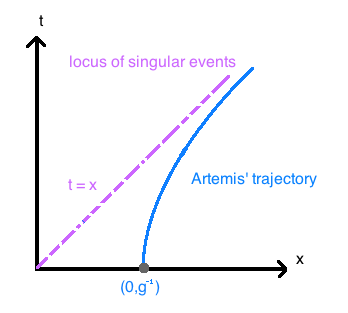
\includegraphics[width=0.5\textwidth]{images/singularities.png}
\caption{Locus of singular events}
\label{singularities diagram}
\end{figure}

The locus of singular events lies on the line $t=x$ in the global inertial frame; that is the ray of a photon emitted at $t=0$. All points along this line map to the origin (as with the coordinate singularity at $x'=g^{-1}$). Physically, the graph shows that all points beyond the dotted line are inaccessible to Artemis; in her reference frame they do not occur.

These singularities arise due to choice of reference frame, and are not inherent to spacetime itself (we could easily imagine reference frames in which events beyond the locus are observed).


\begin{framed}
\textbf{v.} Show that the only nonzero Christoffel symbols in the primed coordinates are
\begin{align}
\Gamma^{0'}_{0'1'}&=g(1+gx')^{-1}=\Gamma^{0'}_{1'0'} \label{Chris 1}\\
\Gamma^{1'}_{0'0'}&=g(1+gx').\label{Chris 2}
\end{align}
\end{framed}

The Christoffel symbols are given by
\begin{equation}
\Gamma^{\lambda}_{\alpha\beta}=\frac{1}{2}g^{\lambda\mu}(g_{\mu\alpha,\beta}+g_{\mu\beta,\alpha}-g_{\alpha\beta,\mu})
\end{equation}
where
\begin{equation}
g_{\alpha\beta,\mu}=\frac{\partial g_{\alpha\beta}}{\partial x^{\mu}}
\end{equation}

The only non-constant component of the metric is $g_{0'0'}=-(1+gx')^2$ which depends only on $x'=x^{1'}$, hence the only non-zero terms $g_{\alpha\beta,\mu}$ is
\begin{equation}
g_{0'0',1'}=\frac{\partial g_{0'0'}}{\partial x^{1'}}=-2g(1+gx')
\end{equation}
and hence the only non-zero Christoffel symbols $\Gamma^{\lambda}_{\alpha\beta}$ require $\{\alpha,\beta,\lambda\}=\{0',0',1'\}, \{0',1',0'\},$ or $\{1',0',0'\}$.

\begin{align}
\Gamma^{1'}_{0'0'}&=\frac{1}{2}g^{1' \mu}(g_{\mu 0',0'}+g_{\mu 0',0'}-g_{0'0',\mu})\\
&=\frac{1}{2}g^{1'1'} (-g_{0'0',1'})\\
&=g(1+gx')\\
\Gamma^{0'}_{1'0'}&=\frac{1}{2}g^{0' \mu}(g_{\mu 1',0'}+g_{\mu 0',1'}-g_{1'0',\mu})\\
&=\frac{1}{2}g^{0'0'}(g_{0'0',1'})\\
&=g(1+gx')^{-1}\\
\Gamma^{0'}_{0'1'}&=\frac{1}{2}g^{0' \mu}(g_{\mu 0',1'}+g_{\mu 1',0'}-g_{0'1',\mu})\\
&=\frac{1}{2}g^{0'0'}(g_{0'0',1'})\\
&=g(1+gx')^{-1}
\end{align}
And so, we have found all the non-zero primed Christoffel symbols!


\begin{framed}
\textbf{(c)} Artemis looks out of the windscreen of her rocket ship and “sees” Diana hovering a constant distance away. (We explore what “sees” means further below.) Putting her ruler and clock in her pocket, she opens the airlock, adjusts the mini-thrusters on her space suit, and heads out (slowly, to avoid introducing unwanted relativistic distortions!) to measure the coordinate distance to her sister. Laying the ruler end to end, she confirms that Diana hovers at rest at the spatial location $(x',y',z')=(h,0,0)$ for all $t'$.
\end{framed}

\begin{framed}
\textbf{i.} Calculate Diana’s 4-velocity in the primed coordinates. You should find
\begin{align}
u^{0'}&=(1+gh)^{-1},\label{ci. eq1}\\
u^{1'}&=0.\label{ci. eq2}
\end{align}
\end{framed}

In flat spacetime, we know
\begin{equation}
\vec{u}=\left(\frac{dt}{d\tau},\frac{dx}{d\tau},\frac{dy}{d\tau},\frac{dz}{d\tau}\right)
\end{equation}
where $\tau$ is the proper time of the object whose velocity is being calculated.

Diana's position in Artemis' reference frame is
\begin{align}
x'_D&=h\\
y'_D&=0\\
z'_D&=0
\end{align}
so Diana's 4-velocity is given by
\begin{equation}
\vec{u}'_D=\left(\frac{dt'}{d\tau_D},\frac{dx'_D}{d\tau_D}, \frac{dy'_D}{d\tau_D}, \frac{dz'_D}{d\tau_D} \right)
=\left(\frac{dt'}{d\tau_D},0,0,0 \right)\label{Diana 4-velocity}
\end{equation}

We also know, by normalisation, that
\begin{equation}
\vec{u}\cdot \vec{u}=-1,
\end{equation}
which is an invariant and hence true in all frames. Hence for Diana's velocity, we have
\begin{align}
-1&=\vec{u}'_D\cdot \vec{u}'_D=g_{tt}(\underbrace{u^{0'}}_{\equiv\frac{dt}{d\tau_D}})^2\\
\Rightarrow u^{0'}&=\left(-\frac{1}{g_{t't'}}\right)^{1/2}\\
&=\left[\frac{1}{(1+gx')^2}\right]^{1/2}\\
&=(1+gx')^{-1}
\end{align}

Since Artemis measures $x'=h$, we conclude Diana's 4-velocity in Artemis' frame to be
\begin{equation}
\vec{u}'=\left[(1+gh)^{-1},0,0,0\right]
\end{equation}



\begin{framed}
\textbf{ii.} Calculate Diana’s 4-acceleration in the primed coordinates. You should find
\begin{align}
a^{0'}&=0,\label{cii. eq1}\\
a^{1'}&=g(1+gh)^{-1}.\label{cii. eq 2}
\end{align}
\end{framed}

Where $\vec{a}'$ is Diana's 4-acceleration in Artemis' frame, and $\vec{u}'$ is Diana's 4-velocity in said frame, we have
\begin{align}
\vec{a}'&=\nabla_{\vec{u}'}\vec{u}'\\
\Rightarrow a^{\alpha'}&=u^{\beta'}\left(\frac{\partial u^{\alpha'}}{\partial x^{\beta'}}
+\Gamma^{\alpha'}_{\lambda\beta'}u^{\lambda}\right)\label{calculate a}
\end{align}

We recall from (\ref{Chris 1}) and (\ref{Chris 2}) that
\begin{align*}
\Gamma^{0'}_{0'1'}&=g(1+gx')^{-1}=\Gamma^{0'}_{1'0'}\\
\Gamma^{1'}_{0'0'}&=g(1+gx')
\end{align*}

We also see that
\begin{equation}
\frac{\partial u^{\alpha'}}{\partial x^{\beta'}}=0
\end{equation}
for all $\alpha'$, since $u^{\alpha'}$ is constant for all $\alpha'$.

Hence from (\ref{calculate a}), we can determine
\begin{align}
a^{0'}&=u^{\beta'}\left(\Gamma^{0'}_{\lambda\beta} u^{\lambda}\right)\\
&=u^{0'}\left(\Gamma^{0'}_{0'0'}u^{0'}\right)+u^{0'}\left(\Gamma^{0'}_{1'0'}u^{1'}\right)+
u^{1'}\left(\Gamma^{0'}_{0'1'}u^{0'}\right)+u^{1'}\left(\Gamma^{0'}_{1'1'}u^{1'}\right)\\
&=0\\
a^{1'}&=u^{\beta'}\left(\Gamma^{1'}_{\lambda\beta} u^{\lambda}\right)\\
&=u^{0'}\left(\Gamma^{1'}_{0'0'}u^{0'}\right)+u^{0'}\left(\Gamma^{1'}_{1'0'}u^{1'}\right)+
u^{1'}\left(\Gamma^{1'}_{0'1'}u^{0'}\right)+u^{1'}\left(\Gamma^{1'}_{1'1'}u^{1'}\right)\\
&=\Gamma^{1'}_{0'0'}\left(u^{0'}\right)^2\\
&=g(1+gx')\cdot (1+gx')^{-2}\\
&=g(1+gh)^{-1},\quad\text{since $x'=h$ at Diana's position}\\
a^{2'}&=u^{\beta'}\left(\Gamma^{2'}_{\lambda\beta} u^{\lambda}\right)\\
&=u^{0'}\left(\Gamma^{2'}_{0'0'}u^{0'}\right)+u^{0'}\left(\Gamma^{2'}_{1'0'}u^{1'}\right)+
u^{1'}\left(\Gamma^{2'}_{0'1'}u^{0'}\right)+u^{1'}\left(\Gamma^{2'}_{1'1'}u^{1'}\right)\\
&=0\\
a^{3'}&=u^{\beta'}\left(\Gamma^{3'}_{\lambda\beta} u^{\lambda}\right)\\
&=u^{0'}\left(\Gamma^{3'}_{0'0'}u^{0'}\right)+u^{0'}\left(\Gamma^{3'}_{1'0'}u^{1'}\right)+
u^{1'}\left(\Gamma^{3'}_{0'1'}u^{0'}\right)+u^{1'}\left(\Gamma^{3'}_{1'1'}u^{1'}\right)\\
&=0\\
\end{align}
which is as expected.

%------------------------------------------------------------------------------------------------------------

\begin{framed}
\textbf{iii.} Explain in words why equations (\ref{ci. eq1}), (\ref{ci. eq2}), (\ref{cii. eq1}) and (\ref{cii. eq 2}) imply that Diana's \emph{proper acceleration} is constant but different from Artemis’s proper acceleration.
\end{framed}

In the primed coordinates, Artemis' 4-acceleration is $\vec{a}'_A=(0,g,0,0)$ while Diana's 4-acceleration is given by $\vec{a}'_D=\left[0,g(1+gh)^{-1},0,0\right]$. A proper acceleration is measured relative to an inertial (non-accelerating) observer or reference frame; as described in 1), Artemis' proper acceleration is $g$.

We can calculate the quantities $\vec{a}\cdot\vec{a}$ for both Artemis' and Diana's accelerations as
\begin{align}
\vec{a}'_A\cdot \vec{a}'_A&=g^2\\
\vec{a}'_D\cdot \vec{a}'_D&=g^2(1+gh)^{-2}
\end{align}

Hence these quanitities $\vec{a}\cdot \vec{a}$ are invariant (in flat spacetime), identical for all coordinate systems. So when calculated in the global inertial reference frame we find
\begin{align}
\vec{a}_A\cdot \vec{a}_A &=g^2\\
\Rightarrow (\text{proper acceleration})_{A}=\lvert\sqrt{\vec{a}_A\cdot \vec{a}_A}\rvert&=g
\intertext{which is Artemis' proper acceleration as quoted previously.}
\vec{a}_D \cdot \vec{a}_D &= g^2(1+gh)^{-2}\\
\Rightarrow (\text{proper acceleration})_{D}=\lvert\sqrt{\vec{a}_D\cdot \vec{a}_D}\rvert&=g(1+gh)^{-1}\label{Diana prop a}
\end{align}
so we observe that Artemis and Diana indeed have constant, but different, proper accelerations.


\begin{framed}
\textbf{iv.} Argue (carefully!) that the proper time $\Delta\tau_D$ between ticks of Diana’s clock on board her rocket ship is related to the proper time $\Delta\tau_A$ between ticks of Artemis’s clock on board her rocket ship according to
\begin{equation}
\frac{\Delta\tau_A}{\Delta\tau_D}=\frac{1}{1+gh}
\end{equation}
\end{framed}

\begin{align}
\frac{\Delta \tau_A}{\Delta \tau_D}&=\frac{d\tau_A}{d\tau_D}\\
&=\frac{d\tau_A}{dt'}\frac{dt'}{d\tau_D}
\intertext{In Artemis' frame, $t'=\tau_A$, so we know}
\frac{d\tau_A}{dt'}&=0
\intertext{To determine $\frac{dt'}{d\tau_D}$, we consider Diana's 4-velocity, $\vec{u}'_D$. This velocity is in Artemis' frame, but looks at motion along Diana's worldline. From (\ref{Diana 4-velocity}) we see the first component is given as $\frac{dt'}{d\tau_D}$, so}
\frac{dt'}{d\tau_D}&=(1+gh)^{-1}\quad\text{from (\ref{ci. eq1})}\\
\Rightarrow \frac{\Delta \tau_A}{\Delta \tau_D}&=1\cdot\left[(1+gh)^{-1}\right]^{-1}\\
&=\frac{1}{1+gh}
\end{align}


\begin{framed}
\textbf{v.} Combine all of the above results to show that Diana’s trajectory in the global inertial frame is given by
\begin{align}
t_D(\tau_D)&=(g^{-1}+h)\sinh[(g^{-1}+h)^{-1}\tau_D],\label{eq21}\\
x_D(\tau_D)&=(g^{-1}+h)\cosh[(g^{-1}+h)^{-1}\tau_D],\label{eq22}
\end{align}
ith departure point $(t,x,y,z)=(0,g^{-1}+h,0,0)$. Please note that there are many valid ways to approach this part of the question, e.g. by transforming the relevant vectors from primed to Minkowski coordinates.
\end{framed}

From a) iii) we have the transformations
\begin{align*}
t&=(g^{-1}+x')\sinh gt, \\
x&=(g^{-1}+x') \cosh gt',\\
y&=y',\\
z&=z'.
\end{align*}

Diana's position in the primed frame is given by
\begin{equation}
\vec{x}'=(\tau_A,h,0,0).
\end{equation}

Recalling that
\begin{align}
\frac{\Delta \tau_A}{\Delta \tau_D}\Rightarrow \tau_A=\frac{1}{1+gh}\tau_D
\end{align}

we find that

\begin{align}
t_D(\tau_A)&=(g+h)\sinh g\tau_A\\
\Rightarrow t_D(\tau_D)&=(g^{-1}+h)\sinh\left[g(1+gh)^{-1}\tau_D\right]\\
&=(g^{-1}+h)\sinh\left[(g^{-1}+h)^{-1}\tau_D\right]\\
x_D(\tau_A)&=(g+h)\cosh g\tau_A\\
\Rightarrow x_D(\tau_D)&=(g^{-1}+h)\cosh \left[g(1+gh)^{-1}\tau_D\right]\\
&=(g^{-1}+h)\cosh \left[(g^{-1}+h)^{-1}\tau_D\right]
\end{align}

Now since $\tau_A\propto \tau_D$, $\tau_A=0\Rightarrow \tau_D=0$. At $\tau_A=0$, Diana's position in the primed coordinates are $(0,h,0,0)$.

\begin{align}
\Rightarrow t_D(0)&=(g^{-1}+h)\sinh 0=0\\
x_D(0)&=(g^{-1}+h)\cosh 0 = g^{-1}+h
\end{align}

Also, since $y=y'$ and $z=z'$, we know
\begin{align}
y_D(0)&=0\\
z_D(0)&=0
\end{align}
hence Diana's departure point in the global inertial reference frame is given by
\begin{equation}
(t,x,y,z)=(0,g^{-1}+h,0,0)
\end{equation}


\begin{framed}
\textbf{(d)} Artemis and Diana conduct a laser ranging experiment with the supplies in their space packs. Back in her own rocket ship, Artemis fires her laser pointer straight at Diana. Diana holds up her mirror and reflects the light ray back to Artemis. Artemis measures the round-trip time in the primed coordinate system and infers the \emph{radar distance}.
\end{framed}

\begin{framed}
\textbf{i.} Show that the path $[t'(\lambda),x'(\lambda)]$ traced by a photon on its way from Artemis to Diana (where $\lambda$ is an affine parameter) satisfies
\begin{equation}
\frac{dt'}{dx'}=\frac{1}{1+gx}\label{di. eq1}
\end{equation}
\end{framed}

We can determine the spacetime interval $ds^2$ from the metric,
\begin{equation}
g(d\vec{x},d\vec{x})=g_{\alpha'\beta}dx^{\alpha'}dx^{\beta'}=ds^2
\end{equation}

For the path traced by the photon, we know $ds^2=0$ since it is a null ray (light travels a path neither spacelike nor timelike). Along the path,
\begin{align}
g_{0'0'}dx^{0'}dx^{0'}+g_{1'1'}dx^{1'}dx^{1'}=0\\
\Rightarrow -(1+gx')^2(dt')^2+(dx')^2&=0\\
\Rightarrow \frac{(dx')^2}{(dt')^2}&=(1+gx')^2\\
\Rightarrow \frac{dt'}{dx'}&=\frac{1}{1+gx'}
\end{align}
as required.



\begin{framed}
\textbf{ii.} From (\ref{di. eq1}), show that the radar distance is given by $g^{-1}\ln (gh+1)$. The radar distance is is always longer than the coordinate distance $h$.
\end{framed}

We first find the time taken for the light to reach Diana.
\begin{equation}
dt'=\frac{dx'}{1+gx'}\Rightarrow t'=\frac{1}{g}\int\frac{dx'}{x'+g^{-1}}=g^{-1}\ln(x'+g^{-1})+C\label{radar time +c}
\end{equation}
where $C$ is a constant.

At $t'=0$, the photon is located at Artemis' position so $x'=0$
\begin{equation}
\Rightarrow 0= g^{-1}\ln(g^{-1})+C=-g^{-1}\ln (g)+C \Rightarrow C= g^{-1}\ln (g)
\end{equation}

Now substituting this into (\ref{radar time +c}),
\begin{align}
t'&=g^{-1}\ln(x'+g^{-1})+g^{-1}\ln(g)\\
&=g^{-1}\ln(1+gx')\\
&=g^{-1}\ln(1+gh)\label{radar time}
\end{align}
since Diana is located at $x'=h$.

The radar distance is the distance travelled by the photon to reach Diana's geodesic, which we calculate as
\begin{equation}
\text{radar distance}=\text{radar time}\cdot\text{photon speed}=g^{-1}\ln(1+gh)\times 1=g^{-1}\ln(1+gh),\label{radar distance}
\end{equation}
as required.



\begin{framed}
\textbf{iii.} Draw a spacetime diagram in Minkowski coordinates, i.e. in the $x-t$ plane, showing the trajectories of Artemis, Diana, and the photon round trip.
\end{framed}

\begin{figure}[h]
\centering
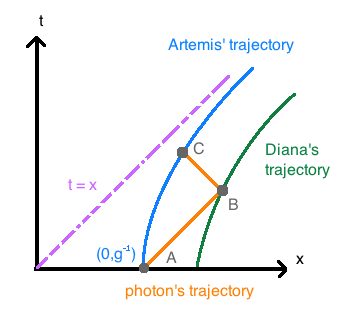
\includegraphics[width=0.4\textwidth]{images/photon_round_trip.png}
\caption{Spacetime diagram of the photon round trip in Minkowski coordinates}
\label{photon round trip figure}
\end{figure}

Note the photon travels with slope = 1 from $\mathcal{A}$ to $\mathcal{B}$, and slope = -1 from $\mathcal{B}$ to $\mathcal{C}$; this is due to the photon travelling at speed $v=1$ (in natural units, of course).

\begin{framed}
\textbf{iv.} Calculate the Minkowski coordinates of the three key events that define the laser ranging experiment: photon emitted by Artemis, photon reflected by Diana, photon received back by Artemis. You should find
\begin{align}
(t,x)&=(0,g^{-1}),\\
(t,x)&=(2g)^{-1}[(1+gh)^2-1,(1+gh)^2+1],\\
(t,x)&=(2g)^{-1}[(1+gh)^2-(1+gh)^{-2},(1+gh)^2+(1+gh)^{-2}].
\end{align}
\end{framed}

We will denote the key events - photon emitted by Artemis, photon reflected by Diana, photon received back by Artemis - as $\mathcal{A}$, $\mathcal{B}$ and $\mathcal{C}$ respectively.

Event $\mathcal{A}$ occurs at Artemis' starting position, which in Minkowski coordinates is written as
\begin{equation}
(t,x)_{\mathcal{A}}=(0,g^{-1})
\end{equation}

\begin{figure}[h]
\centering
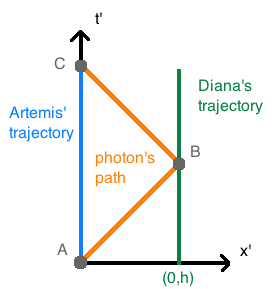
\includegraphics[width=0.4\textwidth]{images/photon_round_trip_primed.png}
\caption{Spacetime diagram of photon round trip in primed coordinates}
\label{photon round trip primed diagram}
\end{figure}

Event $\mathcal{B}$ occurs when the photon reaches Diana. Since Diana is always located at $x'=h$ and the time taken by the photon to reach Diana is $t'=g^{-1}\ln(1+gh)$ from (\ref{radar time}), we have
\begin{equation}
(t',x')_{\mathcal{B}}=(g^{-1}\ln(1+gh),h)
\end{equation}
Let's transform this to Minkowski coordinates.
\begin{align}
t&=(g^{-1}+h)\sinh\left[\log(1+gh)\right]\\
&=g^{-1}(1+gh)\left[\frac{1+gh-\frac{1}{1+gh}}{2}\right]\\
&=g^{-1}\cancel{(1+gh)}\left[\frac{(1+gh)^2-1}{2 \cancel{(1+gh)}}\right]\\
&=(2g)^{-1}\left[(1+gh)^2-1\right]
\intertext{}
x&=(g^{-1}+h) \cosh \left[\log(1+gh)\right]\\
&=g^{-1}(1+gh)\left[\frac{1+gh+\frac{1}{1+gh}}{2}\right]\\
&=g^{-1}\cancel{(1+gh)}\left[\frac{(1+gh)^2+1}{2 \cancel{(1+gh)}}\right]\\
&=(2g)^{-1}\left[(1+gh)^2+1\right]
\end{align}
So for event $\mathcal{B}$ we have
\begin{equation}
(t,x)_{\mathcal{B}}=(2g)^{-1}\left[(1+gh)^2-1,(1+gh)^2+1\right]
\end{equation}

From Figure \ref{photon round trip primed diagram}, we see that the photon travels the radar distance again from event $\mathcal{B}$ to event $\mathcal{C}$; hence
\begin{equation}
(t',x')_{\mathcal{C}}=(2g^{-1}\ln(1+gh),0)
\end{equation}
As with event $\mathcal{B}$, we shall transform this into Minkowski coordinates.
\begin{align}
t'&=g^{-1}\sinh\left[g^{-1}\cdot2g^{-1}\log(1+gh)\right]\\
&=g^{-1}\sinh \big[ \log\left[(1+gh)^2\right] \big] \\
&=g^{-1}\left[ \frac{(1+gh)^2-\frac{1}{(1+gh)^2}}{2}\right]\\
&=(2g)^{-1}\left[(1+gh)^2-(1+gh)^{-2}\right]
\intertext{}
x'&=g^{-1} \cosh \left[g^{-1}\cdot2g^{-1}\log(1+gh)\right]\\
&=g^{-1}\cosh \big[ \log\left[(1+gh)^2\right] \big] \\
&=g^{-1}\left[ \frac{(1+gh)^2+\frac{1}{(1+gh)^2}}{2}\right]\\
&=(2g)^{-1}\left[(1+gh)^2+(1+gh)^{-2}\right]
\end{align}
Hence for event $\mathcal{C}$ we find
\begin{equation}
(t,x)_{\mathcal{C}}=(2g)^{-1}\left[(1+gh)^2-(1+gh)^{-2}\,(1+gh)^2+(1+gh)^{-2}\right]
\end{equation}
as required.





\begin{framed}
\textbf{(e)} Encouraged by the laser ranging results, the sisters attempt a ``speed camera'' experiment. Before blasting off in their rocket ships, they compare notes while at rest in the global inertial frame and agree that the proper frequency of the laser pointer is $\nu_e$. Once in flight, Artemis fires her laser pointer at Diana, and Diana reflects the light ray back to Artemis. Both sisters look for a Doppler shift in the frequency of the light ray they receive.
\end{framed}

\begin{framed}
\textbf{i.} Write down Artemis's and Diana's 4-velocities in the primed coordinates.
\end{framed}

\begin{align}
\vec{u}'_A&=(1,0,0,0)\\
\vec{u}'_D&=\left[(1+gh)^{-1},0,0,0\right]
\end{align}

\begin{framed}
\textbf{ii.} Hence, or otherwise, prove that the frequency $\nu_D$ that Diana measures in the proper frame of her rocket ship is given by
\begin{equation}
\frac{\nu_D}{\nu_e}=\frac{1}{1+gh}\label{eii. eq1}
\end{equation}
\end{framed}

We know the 4-momentum of the photon emitted by Artemis is
\begin{equation}
\vec{p}''_{A}=(h_p\nu_e,h_p\nu_e,0,0)
\end{equation}
where $\nu_e$ is the frequency of the photon as seen by Artemis as it is emitted, and $h_p$ is the Planck constant (with subscript $p$ to distinguish it from the distance $h$). The 4-momentum of the photon as seen by Diana is
\begin{equation}
\vec{p}'_{D}=(h_p\nu_D,h_p\nu_D,0,0)
\end{equation}

The quantity $\vec{u}\cdot\vec{p}$ is a Lorentz invariant; that is,
\begin{equation}
\vec{u}\cdot \vec{p}=-E
\end{equation}
where $E$ is the photon energy. Since this is an invariant, it is true in all frames at all points in spacetime. So we have
\begin{align}
\vec{u}'_A \cdot \vec{p}'_A&=-(1+gx')^2 h_p\nu_e\\
&=-h_p\nu_e, \quad\text{since $x'=0$ at Artemis' location}\\
&=-E,
\end{align}
noting the use of the metric in primed coordinates.

At Diana's position in the primed coordinates,
\begin{align}
\vec{u}'_D \cdot \vec{p}'_D &=-(1+gx')^2\cdot(1+gh)^{-1} h_p\nu_D\\
&=-(1+gh)^2\cdot(1+gh)^{-1} h_p\nu_D, \quad\text{since $x'=h$ at Diana's location}\\
&=-(1+gh)^{-1} h_p\nu_D\\
&=-E
\end{align}

Equating these energies, we find
\begin{align}
-(1+gh)^{-1} h_p\nu_D&=-h_p\nu_e\\
\Rightarrow \frac{\nu_D}{\nu_e}&=\frac{1}{1+gh}\label{doppler shift}
\end{align}
as required.



\begin{framed}
\textbf{iii.} Equation (\ref{eii. eq1}) says that Diana observes a nonzero Doppler shift. Yet Artemis and Diana are both at rest in the primed coordinates. Resolve this apparent paradox in physical terms.
\end{framed}

One way to explain the apparent paradox of Artemis and Diana and the Doppler shift is to utilise the equivalence principle: that one cannot distinguish between the effects of a uniform gravitational field on a observer and the effects of a (non-gravitational) constant acceleration. Hence we could consider Artemis and Diana to be under the effect of uniform (though different) gravitational fields.

After the photon is emitted from Artemis, it must travel through a rising gravitational field to reach Diana; as it travels it is gravitationally redshifted! This leads to a decrease in frequency (by factor $(1+gh)^{-1}$ as calculated in (\ref{doppler shift})) as it reaches Diana. After it is reflected and travels back to Artemis, the photon travels through a decreasing gravitational field and is hence gravitationally blueshifted! This of course increases the photon's frequency, such that when it reaches Artemis she measures an unchanged frequency. Though both Artemis and Diana are at rest in the primed coordinates, travelling in a non-inertial frame gives rise to this apparent paradox.


\end{document}







